\section{Introduction}\label{sec:introducao}

In the generations leading up to the fifth generation of wireless cellular mobile networks, the supreme effort was made in the massification of access to customers and increasing the transmission rates. However, more than just improving bandwidth and reducing latency, 5G networks~\cite{shafi:17} will allow truly disruptive solutions to emerging in all types of industries~\cite{kaloxylos:18}. Although many countries, such as Brazil, are still discussing and preparing for the deployment of 5G networks, since 2019, several countries (\textit{e.g.}, China, South Korea, and the United States) are already implementing, testing, and effectively using the latest generation of mobile wireless networks. More than 2.4 billion devices are expected to use 5G networks by 2025~\cite{richter:19}. For now, rates close to (and even higher than) 1~Gbps are still the main novelties, but several services, mainly based on Internet of Things (IoT), began to be planned and implemented. Autonomous cars, Industry 4.0, and virtual/augmented/mixed reality are some of the bets for relevant applications and tend to serve as interesting use cases for new network features. However, as in previous generations, it is difficult to predict accurately which applications or services will be adopted. For the time being, the only consensus is that 5G networks, when deployed on a significant scale, will represent a new step for wireless communications and will have a deep impact in the society~\cite{wef:20}.

The fifth-generation represents a remarkable technological leap over the fourth generation, introducing significant hardware and, above all, considerable software innovations. It is essential to clarify that this leap hides the various intermediate steps that comprise it. In the telecommunications industry, including for advertising reasons, a significant amount of technological developments and innovations accumulate before defining a generation, which was no different at 5G networks. As an example, the Releases provided by the 3GPP (3rd Generation Partnership Project) that is one of the leading organizations for standardizing wireless mobile networks. The 4G/LTE networks (Long-Term Evolution) were introduced in 2008 by Release 8~\cite{3GPP-rel08:19} and, since then, have received several updates (represented by new Releases) until the 5G networks were officially introduced by Release 15~\cite {3gpp:rel15nr21.915} in 2018. On the other hand, there are technical factors that also support the definition of each generation. In the 5G system, the radio spectrum usage is expanding to hundreds of MHz or some units of GHz, but it also going to frequency bands of tens of GHz. Moreover, 5G networks consolidate an intense process of softwarization that stands out for the adoption of cloud systems and technologies such as virtualization~\cite{abdelwahab:16}, software-defined networks~\cite{chen:15}, network slicing~\cite{foukas2017network}, and Service-Based Architecture (SBA)~\cite{mademann:18}.

In addition to the technological aspects, the 5G networks introduce changes in the companies' business model. Traditionally, operators of wireless mobile communication systems have focused on end-users as the main sources of revenue. In 5G networks, the intention is to expand (or even migrate) the focus to have industries as primary customers~\cite{palattella:16,lema:17}. Three main requirements (or scenarios) have been defined to support this expansion of the telecommunications companies' business model: enhanced mobile broadband (eMBB), ultra-reliable low-latency communications (URLLC), and massive machine-type communications (mMTC). These scenarios are illustrated in Fig.~\ref{subfig:cenarios_5g}, which was introduced by ITU (International Telecommunication Union)~\cite{itu:15}, in 2015, as part of the vision of what 5G networks would be. This illustration, which presents the leading capabilities of each scenario, is widely used to try to summarize some relevant properties of 5G networks.

\begin{figure}[htb]
\centering
    \subfigure[5G scenarios]
    {\label{subfig:cenarios_5g}
    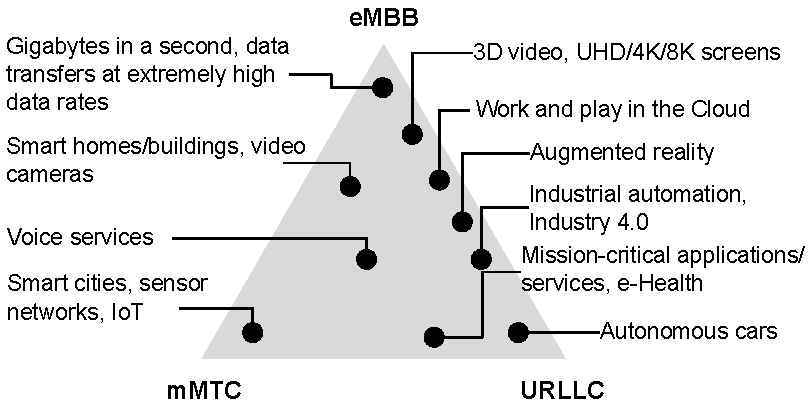
\includegraphics[width=.48\textwidth]{figs/cenarios_5G_eng.pdf}}
    \hfil
    \subfigure[Capabilities of the scenarios]
    {\label{subfig:capacidades_cenarios_5g}
    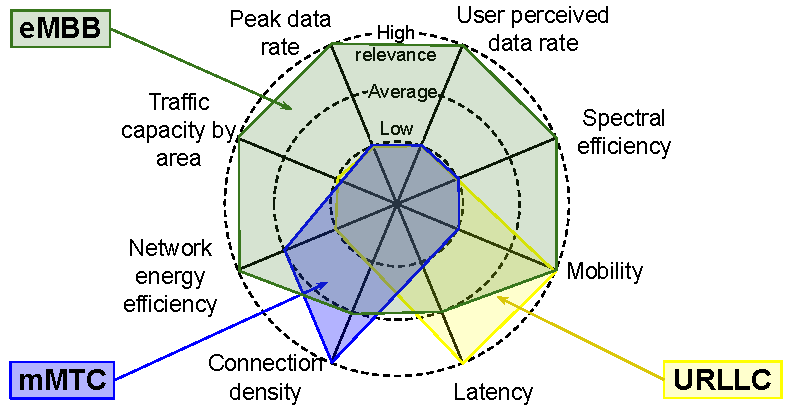
\includegraphics[width=.48\textwidth]{figs/capacidades_cenarios_5G_eng.pdf}}
    \caption{Scenarios (or requirements) defined for 5G networks (left) and capabilities offered in these scenarios (right).}
\label{fig:redes_5g}
\end{figure}

In order to meet the requirements of the different scenarios, the concepts of network software began to be adopted, both by academia and industry, to make the development of 5G networks (or systems) viable in recent years and also their evolution~\cite{foukas2017network}. The main reason for the intensive introduction of software in 5G systems is to extend the flexibility to the mobile network architecture, supporting different requirements in challenging scenarios emerging in the digitalized society. Moreover, with the network softwarization, it is possible to enjoy of traditional cloud computing, as well as its smaller-scale variants, \textit{i.e.}, fog and edge. In this context, radio access and core network functions are now implemented using the advantages of cloud computing, such as abundant storage, large-scale processing, elasticity, etc. In addition to enable new services, in the long run, the softwarization is expected to reduce the costs of deploying and operating 5G systems.

The remainder of this article is structured as follows. Section~\ref{sec:redesMoveis} introduces basic concepts related to mobile network cellular networks and the operation of this type of system. This section presents a brief historic review of the generations until the forth. Section~\ref{sec:5G} is focused in the fifth generation and its evolution. Some key technologies, mainly related to software, are presented in this section. In the Section~\ref{sec:RAN}, the Radio Access Network (RAN) is presented in more detail and some aspects of softwarization process is discussed. Section~\ref{sec:core} describe the 5G core and most of the several functions that compose the new architecture. In the Section~\ref{sec:integracao}, some aspects of the integration of a 5G system and non-3GPP access networks are presented. This section also discuss in more detail the integration of a 5G core and LoRa access networks. Finally, Section~\ref{sec:conclusao} summarizes the contributions expected in the Releases 16 and 17, mainly in the software context.